\documentclass{book}

\usepackage{tikz}
\usepackage[bottom]{footmisc}
\usepackage{listings}
\usepackage[inner=1in, outer=0.25in, top=1in, bottom=1in]{geometry}
\usepackage{hyperref}
\usepackage{fancyhdr}
\usepackage{lastpage}
\usepackage[dvipsnames]{xcolor}


\newcommand{\bold}[1]{\textbf{#1}}
\newcommand{\italic}[1]{\textit{#1}}

\pagestyle{fancy}

\fancyhead[L]{}

\pagenumbering{roman}

\renewcommand{\headrulewidth}{2pt}
\renewcommand{\footrulewidth}{2pt}

\begin{document}

	\begin{titlepage}
		\begin{center}
			\Huge\bold{Tikz Basics}\\
			\huge\bold{Graphics in \LaTeX}
			
			\vfill
			
			\Large\textsc{Written By}\\
			\Large\bold{Priyanuj Bora}
			
			\vfill
			
			October 10 2024
		\end{center}
	\end{titlepage}
	
	\tableofcontents
	
	\chapter{Introduction}
	\label{ch:ch1}
	\setcounter{page}{1}
	\pagenumbering{arabic}
	\fancyhead[L]{\leftmark}
	\fancyhead[R]{\rightmark}
	\fancyfoot[R]{Page \thepage\ of \pageref{LastPage}}
	\fancyfoot[C]{}
	\paragraph{}
	
	The \emph{tikz} package is used when we want to draw some diagrams in \LaTeX.
	
	In order to use it, we first need to include it using the the \lstinline|\usepackage{}| command like so:
	
\begin{lstlisting}[frame=tlBR]
\documentclass{.....}
....
....
....
\usepackage{tikz}
....
....
....
\end{lstlisting}
	
	To be able to draw using this package, we need to use an environment called \lstinline|tikzpicture| like so:
	
\begin{lstlisting}[frame=tlBR]
\begin{tikzpicture}
% write your code here
\end{tikzpicture}
\end{lstlisting}

\section{Drawing a simple line}
\label{sec:sec1}
\paragraph{}

To draw a simple line, use the following command:

\begin{lstlisting}[frame=tlBR]
\begin{tikzpicture}
	\draw(0,0)--(3,3);
\end{tikzpicture}
\end{lstlisting}

The dashes \lstinline|--| between $(0,0)$ and $(3,3)$ indicate that we want a line.

\bold{NOTE}: Don't forget the \italic{semicolon} \lstinline|;|

Here's the \href{https://github.com/0x50-0x42/latex/blob/LaTeX/Tikz/codes/simpleLine.tex}{\textcolor{blue}{Code}}.

Here's the \href{https://github.com/0x50-0x42/latex/blob/LaTeX/Tikz/codes/simpleLine.pdf}{\textcolor{blue}{Output}}.

\section{Drawing zig-zag lines}
\paragraph{}

Now, we will use the same code that we used in \bold{\nameref{sec:sec1}}, but will be longer now.

\begin{lstlisting}[frame=tlBR]
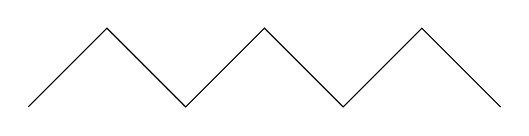
\begin{tikzpicture}
	\draw(0,0)--(1,1)--(2,0)--(3,1)--(4,0)--(5,1)--(6,0);
\end{tikzpicture}
\end{lstlisting}

Here's the \href{https://github.com/0x50-0x42/latex/blob/LaTeX/Tikz/codes/zig_zag.tex}{code}.

Here's the \href{https://github.com/0x50-0x42/latex/blob/LaTeX/Tikz/codes/zig_zag.pdf}{output}.

Notice the \emph{semicolon} being used at the end.

\section{Drawing triangle}
\paragraph{}

A triangle is a closed figure, so we need to use an extension \lstinline|--cycle| to close the figure. Basically it will draw a line from the last coordinate to the first coordinate, thus adding the last side to the figure.

\begin{lstlisting}[frame=tlBR]
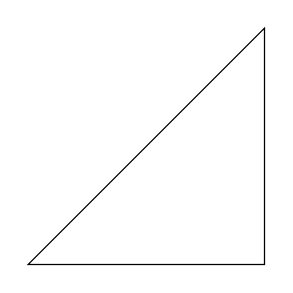
\begin{tikzpicture}
	\draw(0,0)--(3,0)--(3,3)--cycle;
\end{tikzpicture}
\end{lstlisting}

Notice that we first join $(0,0)$ with $(3,0)$ and then we join $(3,0)$ with $(3,3)$. Finally, we use \lstinline|--cycle| to join $(3,3)$ with $(0,0)$ which eventually forms a triangle.

Here's the \href{https://github.com/0x50-0x42/latex/blob/LaTeX/Tikz/codes/triangle.tex}{code}.

Here's the \href{https://github.com/0x50-0x42/latex/blob/LaTeX/Tikz/codes/triangle.pdf}{output}.

\end{document}